\documentclass[reqno]{amsart}

\usepackage{external/takodachi}

\renewcommand{\emph}{\textsc}

% Title: change problem set number as needed
\title
{
	\emph{Littlewood-Paley theory of function spaces}
} 

\author{Jason Zhao}
\date{\today}

\begin{document}
\maketitle

\begin{abstract}
	We present an approach to function spaces based on frequency space localisations. This approach reduces the classical results of Sobolev embedding and traces to elementary Littlewood-Paley theory and interpolation. We draw primarily from \cite{Triebel1983}, \cite{BahouriEtAl2011}, \cite{WangEtAl2011}, and \cite{Grafakos2014a}. 
\end{abstract}

\tableofcontents

\section{Preliminaries}

\subsubsection*{Geometry of Minkowski space}
Let $(\R^{1 + d}, \bfm)$ denote $(1 + d)$-dimensional Minkowski space with the usual metric, which in rectilinear coordinates $(t, x^1, \dots, x^d)$ takes the diagonal form 
	\[ 
		\bfm = - (\d t)^2 + (\d x^1)^2 + \dots + (\d x^d)^2. 
	\]
We will often write $t = x^0$ for the time coordinate and $x = (x^1, \dots, x^d)$ for the spatial coordinates. We reserve Greek indices, such as $\alpha, \beta, \gamma, \dots$ for space-time coordinates $(t, x^1, \dots, x^d)$, while Latin indices, such as $i, j, k, \ell,\dots$ will be reserved for spatial coordinates $(x^1, \dots, x^d)$. Another useful choice are the polar coordinates $(t, r, \Theta)$ where $r = |x|$ denotes the radius from the origin, and $\Theta := x/|x|$ denotes the radial projection onto the unit sphere $\SS^{d - 1}$. In these coordinates, the Minkowski metric takes the form 
	\[
		\bfm = - \d t^2 + \d r^2 + r^2 g_{\SS^{d - 1}}.
	\]
Denote $\partial_r = \tfrac{x^j}r \partial_j$ the radial vector field and $\nabla_{\SS^{d - 1}}$ for the gradient on the unit sphere $\SS^{d - 1}$. 

\subsubsection*{Geometry of the light cone}

We now introduce notation for the geometry of the light cone and subsets thereof. First and foremost, the forward light cone is defined by 
	\[
		C := \{ (t, x) \in [0, \infty) \times \R^d : r \leq t \}. 
	\]
When studying the light cone, it is convenient to work in null coordinates $(u, v, \Theta)$ defined by $u = t - r$ and $v = t + r$. In these coordinates, the Minkowski metric takes the form 
	\[
		\bfm = - \d u \d v + r^2 g_{\SS^{d -1}}.
	\]
The coordinate vector fields $L = \partial_t + \partial_r = 2 \partial_v$ and $\underline L = \partial_t - \partial_r = 2 \partial_u$ are referred to as null vector fields, as they are parallel to the forward and backwards light cones respectively. Observing that the forward light cone is foliated by surfaces
	\[
		\HH^d_{\rho} := \{ (t, x) \in [0, \infty) \times \R^d : t^2 + r^2 = \rho^2 \},
	\]
we introduce hyperbolic coordinates $(\rho, y, \Theta)$ where $\rho = \sqrt{t^2 - r^2}$ and $y = \tanh^{-1} (r/t)$. Each surface $\HH^d_\rho$ is isometric to the simply connected space of constant sectional curvature $-\tfrac{1}{\rho^2}$. In these coordinates the Minkowski metric takes the form 
	\begin{align*}
		\bfm 
			&= - \d \rho^2 + \rho^2  g_{\HH^d_\rho}\\
			&= - \d \rho^2 + \rho^2 (\d y^2 + \sinh^2 (y) g_{\SS^{d - 1}}).
	\end{align*}
We refer to the vector field $S = \rho \partial_\rho = x^\mu \partial_\mu$ as the scaling vector field, as it is generated from the scaling symmetry of the linear wave equation. 

	\begin{figure}[ht]
		\begin{center}
			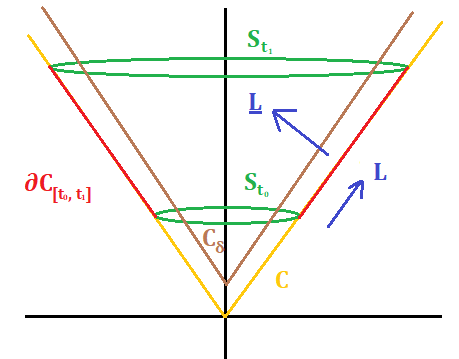
\includegraphics{graphics/cone}
			\caption{The geometry of the light cone. As a wise man once said, a picture is worth $\tfrac1\epsilon$-words for $\epsilon \ll 1$. }
		\end{center}	
	\end{figure}		

\subsubsection*{Subsets of $\R^d$ and $\R^{1 + d}$}
Define the restriction of the light cone to a time interval $I \subseteq [0, \infty)$ and a time slice $t \in [0, \infty)$ respectively by
	\begin{align*}
		C_I 
			&:= C \cap (I \times \R^d), \\
		S_{t}
			&:= C \cap (\{t\} \times \R^d).
	\end{align*}
The \emph{null boundary} $\partial C_I$ denotes the boundary of the time-slab $C_I$ modulo the top and bottom time-slices. Due to singularities on the null boundary, we will also consider the shifted light cone 
	\[ C^\delta := (\delta, 0) + C. \]
Accordingly, we have 
	\begin{align*}
		C^\delta_I
			&:= C_I \cap C^\delta, \\
		S^\delta_t
			&:= S_t \cap C^\delta.		
	\end{align*}	
We also define $B_r (x) \subseteq \R^d$ to be the ball of radius $r$ centered at $x$. 



\section{Besov spaces}
Let $1 \leq p, q \leq \infty$ and $s \in \R$, we define the \emph{homogeneous Besov space} $\dot B^{s, p}_q (\R^d)$ as the completion of the homogeneous Schwartz space $\dot \cS (\R^d)$ with respect to the norm 
	\[ ||u||_{\dot B^{s, p}_q} := \left|\left| || N^s u_N ||_{L^p_x} \right|\right|_{\ell^q_N (2^\Z)} =  \left( \sum_{N \in 2^\Z} || N^s u_N ||_{L^p}^q \right)^{1/q}, \]
with the usual modification at the endpoints $p, q = \infty$. For the same range of exponents, we analogously define the \emph{inhomogeneous Besov space} $B^{s, p}_q (\R^d)$ as the completion of Schwartz space $\cS (\R^d)$ with respect to the norm 
	\[ ||u||_{B^{s, p}_q} := ||u_{\leq 1}||_{L^p} + \left|\left| || N^s u_N ||_{L^p_x} \right|\right|_{\ell^q_N (2^\N)} =  ||u_{\leq 1}||_{L^p} + \left( \sum_{N \in 2^\N} || N^s u_N ||_{L^p}^q \right)^{1/q}.\]

\subsection{Properties}

We can read off some basic properties of Besov spaces from the definitions and properties of $L^p$-spaces and $\ell^q$-spaces. 

\begin{proposition}[Monotonicity in $s$ and $q$]
	Let $1 \leq p \leq \infty$ and $s \in \R$. 
\begin{enumerate}
	\item For $1 \leq q_1 \leq q_2 \leq \infty$, we have
			\begin{align*}
				||u||_{B^{s, p}_{q_2}} 
					&\lesssim_{q_1, q_2} ||u||_{B^{s, p}_{q_1}},\\
				||u||_{\dot B^{s, p}_{q_2}} 
					&\lesssim_{q_1, q_2} ||u||_{\dot B^{s, p}_{q_1}}.
			\end{align*}
		In particular, we have the continuous embeddings $B^{s, p}_{q_1} (\R^d) \hookrightarrow B^{s, p}_{q_2} (\R^d)$ and $\dot B^{s, p}_{q_1} (\R^d) \hookrightarrow \dot B^{s, p}_{q_2} (\R^d)$. 
	
	\item For $1 \leq q_1, q_2 \leq \infty$ and $\alpha > 0$, we have
			\begin{align*}
				||u||_{B^{s, p}_{q_2}} \lesssim_\alpha ||u||_{B^{s + \alpha, p}_{q_1}}.
			\end{align*}
		In particular, we have the continuous embedding $B^{s + \alpha, p}_{q_1} (\R^d) \hookrightarrow B^{s, p}_{q_2} (\R^d)$.
		
\end{enumerate}\label{prop:basicembedbesov}	
\end{proposition}

\begin{proof}
\leavevmode
\begin{enumerate}
	\item This follows immediately from the embedding $\ell^{q_1} \hookrightarrow \ell^{q_2}$ and the definition of the Besov norms. 
	
	\item By (a), it suffices to prove the result for $q_1 = \infty$ and $q_2 = 1$. We can write
		\begin{align*}
			 \sum_{N \in 2^\N}   ||N^s u_N||_{L^p} 
				&\leq  \Big| \Big| N^{s + \alpha} ||u_N||_{L^p} \Big|\Big|_{\ell^\infty_N (2^\N)}  \sum_{N \in 2^\N}  N^{-\alpha}  \lesssim \Big| \Big| N^{s + \alpha} ||u_N||_{L^p} \Big|\Big|_{\ell^\infty_N (2^\N)},
		\end{align*}	
		as desired. 
\end{enumerate}
\end{proof}

The index $s$ measures \textit{regularity}, as such we should expect the Besov norm to measure the norms of derivatives, for example the \emph{Riesz potential} $|\nabla|^s$ and the \emph{Bessel potential} $\langle \nabla \rangle^s$. When these differential operators are applied to a Littlewood-Paley piece $P_N u$, we see that in frequency space they are comparable to multiplication by $N^s$ and $\langle N\rangle^s$ respectively. This is made rigorous by the following lemma: 

\begin{lemma}[Sobolev-Bernstein inequalities] Let $1 \leq p \leq \infty$ and $s \in \R$. Then 
				\begin{align*}
					|| |\nabla|^s u_N||_{L^p} 
						&\sim N^s ||u_N||_{L^p}, \\
					|| \langle\nabla\rangle^s u_{N}||_{L^p} 
						&\sim \langle N\rangle^s ||u_{N}||_{L^p}.
				\end{align*}			
\end{lemma}

\begin{proposition}[Lifting property]
	Let $1 \leq p , q\leq \infty$ and $s, \sigma \in \R$. Then 
		\begin{align*}
			|||\nabla|^\sigma u||_{\dot B^{s - \sigma, p}_q}
				&\sim ||u||_{\dot B^{s, p}_q}\\
			 || \langle \nabla \rangle^\sigma u ||_{B^{s - \sigma, p}_q} 
			 	&\sim ||u||_{B^{s, p}_q} ,
		\end{align*}	 
	That is, $|\nabla|^\sigma : 	\dot B^{s - \sigma, p}_q (\R^d) \to \dot B^{s, p}_q (\R^d)$ and $\langle \nabla \rangle^\sigma : 	B^{s - \sigma, p}_q (\R^d) \to B^{s, p}_q (\R^d)$ isomorphically. 
\end{proposition}

\begin{proof}
	Immediate from Sobolev-Bernstein. 
\end{proof}

The expected duality relations hold for Besov spaces; the proofs are essentially identical to that for Lebesgue spaces and Sobolev spaces. Denote $1 \leq p', q' \leq \infty$ the dual exponents for $1 \leq p, q \leq \infty$, i.e.
	\[ \frac1p + \frac{1}{p'} = \frac1q + \frac{1}{q'} = 1. \]

\begin{theorem}[Duality]
	Let $1 \leq p, q < \infty$ and $s \in \R$, then 
		\begin{align*}
			\dot B^{s, p}_{q} (\R^d)^* 
				&\cong \dot B^{-s, p'}_{q'} (\R^d), \\
			B^{s, p}_{q} (\R^d)^* 
				&\cong  B^{-s, p'}_{q'} (\R^d).
		\end{align*}
\end{theorem}

\begin{proof}\cite[Theorem 2.11.2]{Triebel1983}
	The inclusion $\dot B^{-s, p'}_{q'} (\R^d) \hookrightarrow \dot B^{s, p}_{q} (\R^d)^* $ is essentially Holder's inequality while the reverse inclusion follows from the identification $\ell^q L^p (2^\Z \times \R^d)^* \cong \ell^{q'} L^{p'} (2^\Z \times \R^d)$ and Hahn-Banach. 
\end{proof}

\subsection{Embeddings}

As with the Sobolev embedding inequalities, the Besov embeddings boil down to a trade of regularity for integrability. Our main tool will be Bernstein's inequality, which states that frequency localisation allows us to move from $L^p$-integrability to $L^q$-integrability at the cost of $(\tfrac{d}{p} - \tfrac{d}{q})$-many derivatives. 

\begin{lemma}[Bernstein's inequalities]
\label{lem:bernstein}
	Let $1 \leq p \leq q \leq \infty$, then 
	\begin{align*}
					||u_N||_{L^q} 
						&\lesssim N^{\frac{d}{p} - \frac{d}{q}} ||u_N||_{L^p}, \\
					||u_{\leq N}||_{L^q} 
						&\lesssim N^{\frac{d}{p} - \frac{d}{q}} ||u_{\leq N}||_{L^p}. 
	\end{align*}
\end{lemma}

\begin{proof}
	Let $1 \leq r \leq \infty$ satisfy $\tfrac1p + \tfrac1r = \tfrac1q + 1$, then by Young's convolution inequality and a change of variables $Nx = y$, we have the inequality
	\begin{align*}
		|| P_N u ||_{L^q} = || u * \widecheck{\psi_N} ||_{L^p} \leq ||u||_{L^p} ||N^d \widecheck \psi(Nx)||_{L^r_x} = N^{d - \frac{d}{r}} ||u||_{L^p} ||\widecheck \psi ||_{L^r_y} \sim N^{\frac{d}{p} - \frac{d}{q}} ||u||_{L^p}.
	\end{align*}
	To obtain $u_N$ instead of $u$ on the right, observe that the same proof holds replacing $P_N$ with the fattened projection $\widetilde{P_N}$. Since $\widetilde{P_N} P_N = P_N$, replacing $u$ with $P_N u$ completes the proof. Arguing similarly furnishes the inequality replacing $u_N$ with $u_{\leq N}$. 
\end{proof}



\begin{theorem}[Homogeneous Besov embedding]
	Let $1 \leq p_1 \leq p_2 \leq \infty$ and $1 \leq q_1 \leq q_2 \leq \infty$ and $s_2 \leq s_1$, then 
		\[ || u ||_{\dot B^{s_2, p_2}_{q_2}} \lesssim || u ||_{\dot B^{s_1, p_1}_{q_1}} \]
	whenever $\frac{s_1}{d} - \frac{1}{p_1} = \frac{s_2}{d} - \frac{1}{p_2}$. In particular, we have the continuous embedding $\dot B^{s_1, p_1}_{q_1} (\R^d) \hookrightarrow \dot B^{s_2, p_2}_{q_2} (\R^d)$.
\end{theorem}

\begin{proof}
	By Proposition \ref{prop:basicembedbesov} (a), it suffices to prove the result for $q_1 = q_2 = q$. Recall Bernstein's inequality, 
		\[ || u_N||_{L^{p_2}} \lesssim N^{\frac{d}{p_1} - \frac{d}{p_2}} ||u_N||_{L^{p_1}}. \]
	Applying the identity $\frac{s_1}{d} - \frac{1}{p_1} = \frac{s_2}{d} - \frac{1}{p_2}$, rearranging, and summing in $\ell^q (2^\Z)$ furnishes the result. 	
\end{proof}

\begin{theorem}[Inhomogeneous embedding]
	Let $1 \leq p_1 \leq p_2 \leq \infty$ and $1 \leq q_1 \leq q_2 \leq \infty$ and $s_2 \leq s_1$, then 
		\[ || u ||_{B^{s_2, p_2}_{q_2}} \lesssim || u ||_{B^{s_1, p_1}_{q_1}} \]
	whenever $\frac{s_1}{d} - \frac{1}{p_1} \geq \frac{s_2}{d} - \frac{1}{p_2}$. In particular, we have the continuous embedding $B^{s_1, p_1}_{q_1} (\R^d) \hookrightarrow B^{s_2, p_2}_{q_2} (\R^d)$.
\end{theorem}

\begin{proof}
	By Proposition \ref{prop:basicembedbesov} (a), it suffices to prove the result for $q_1 = q_2 = q$. Control over the low frequency term $u_{\leq 1}$ follows from Bernstein's inequality. For high frequencies $N \in 2^\N$, we can apply the inequality $\frac{s_1}{d} - \frac{1}{p_1} \geq \frac{s_2}{d} - \frac{1}{p_2}$ with Bernstein's inequality to write 
		\[ || u_N||_{L^{p_2}} \lesssim N^{\frac{d}{p_1} - \frac{d}{p_2}} ||u_N||_{L^{p_1}} \leq N^{s_1 - s_2} ||u_N||_{L^{p_1}}. \]
	Rearranging and summing in $\ell^q (2^\N)$ furnishes the result. 	
\end{proof}

\subsection{Traces}

In the interest of solving boundary value problems, we study the boundedness properties of the \emph{trace} operator $T$ which sends a function $u : \R^d \to \C$ to its restriction on a hyperplane $u_{|x_d = 0} : \R^{d - 1} \to \C$, 
	\[ T u (x') := u(x', 0) = \langle u, \delta_{x_d = 0} \rangle \]
where we use the notation $x = (x_1, \dots, x_d)$ and $x' = (x_1, \dots, x_{d - 1})$. We similarly denote $\cF'$ the Fourier transform and $P_N'$ the Littlewood-Paley projections on the hyperplane $\R^{d - 1}$. As always, the main ingredient for studying the trace operator on Besov spaces is the uncertainty principle. This is encapsulated by the following two lemmas: 

\begin{lemma}
	Given a tempered distribution $u \in \cS' (\R^d)$, the trace of the Littlewood-Paley projection $P_{\leq N} u$ has Fourier support in $|\xi'| \lesssim N$. In particular, 
		\[ P'_M T P_{\leq N} u = 0 \]
	for $M \gtrsim N$. 
\end{lemma}

\begin{proof}
	From the uncertainty principle, restricting to a point in physical space is equivalent to integrating in frequency space, that is, $\langle \delta_0, \phi \rangle = \langle 1, \widehat \phi \rangle$. Moreover, the composition of the Fourier transform on $\R^{d - 1}_{x'}$ with the Fourier transform on $\R_{x_d}$ gives the Fourier transform on $\R^d_x$. Hence, in frequency space
		\[ \cF' T P_{\leq N} u = \cF' P_{\leq N} u (\xi', 0) = \int_\R \cF P_{\leq N} u \, d\xi_d. \]
	As $\cF P_{\leq N} u$ is supported in the ball $|\xi| \lesssim N$, we see that $T P_N u$ has Fourier support in the ball $|\xi'| \lesssim N$. 	
\end{proof}

\begin{lemma}
	Given a tempered distribution $u \in \cS' (\R^d)$, the trace of the Littlewood-Paley projection $P_{\leq N} u$ satisfies
		\[ || TP_{\leq N} u ||_{L^p (\R^{d - 1}_{x'})} \lesssim N^{\frac1p} ||P_{\leq N} u||_{L^p (\R^d_x)} \]
\end{lemma}

\begin{proof}
	Since $\cF P_{\leq N} u$ is supported in $|\xi| \lesssim N$, we see that $\cF_{x_d} P_{\leq N} u$ is supported in $|\xi_d| \lesssim N$ for each fixed $x' \in \R^{d - 1}$. Thus by Minkowski's integral inequality and Bernstein's inequality in one-dimension, 
		\begin{align*}
			||T P_{\leq N} u||_{L^p (\R^{d - 1}_{x'})}
				&\leq \left|\left| || P_{\leq N} u||_{L^\infty (\R_{x_d})} \right|\right|_{L^p (\R^{d - 1}_{x'})} \\
				&\lesssim  \left|\left| N^{\frac1p} || P_{\leq N} u||_{L^p (\R_{x_d})} \right|\right|_{L^p (\R^{d - 1}_{x'})} = N^{\frac1p} ||P_{\leq N} u||_{L^p (\R^d_x)}.
		\end{align*}
	This completes the proof. 	
\end{proof}
	
\begin{theorem}[Besov trace theorem]
	Let $1 < p < \infty$ and $1 \leq q \leq \infty$ and $s > \tfrac1p$, then the trace map satisfies
		\[ ||T u||_{\dot B^{s - \frac1p, p}_q (\R^{d - 1})} \lesssim ||u||_{\dot B^{s, p}_q (\R^d)}. \]
	In particular, it extends to a bounded linear operator $T : \dot B^{s, p}_q (\R^d) \to \dot B^{s - \frac1p, p}_q (\R^{d - 1})$. The analogous results also hold for the inhomogeneous Besov spaces. 
\end{theorem}

\begin{proof}
	We perform a Littlewood-Paley decomposition $u = \sum_N P_N u$. By linearity, we can write $P'_M T u = \sum_N P'_M T P_N u$. Applying the triangle inequality, the previous two lemmas, and boundedness of the projections, we estimate
		\begin{align*}
			||P'_M Tu||_{L^p (\R^{d-1}_{x'})}
				&\lesssim \sum_{N : M \lesssim N} ||P'_M T P_N u||_{L^p (\R^{d - 1}_{x'})}\\
				&\lesssim \sum_{N : M \lesssim N} N^{1/p} ||P_N u||_{L^p (\R^d_x)}.
		\end{align*}		
	Multiplying both sides by $M^{s- 1/p}$ and taking $\ell^q$-norms, this reduces the problem to showing boundedness of the linear operator $A : \ell^q (2^\Z) \to \ell^q (2^\Z)$ defined as
		\[ A (\{ c_N\}_{N \in 2^\Z})_M := \sum_{N : M \lesssim N} N^{\frac1p - s} M^{s - \frac1p} c_N. \]
	Taking $c_N := N^s ||P_N u||_{L^p}$ completes the proof. By Schur's test, we simply need to show that the corresponding kernel of the operator $K(N, M) := \mathbb 1_{N \lesssim M} N^{1/p - s} M^{s - 1/p}$ is uniformly summable in $N$ and $M$. Indeed
	\begin{align*}
		\sum_{N \in 2^\Z}K (N, M) \sim  \sum_{N : N \lesssim M} N^{\frac1p - s} M^{s - \frac1p} \sim 1, \\
		\sum_{M \in 2^\Z}K (N, M) \sim  \sum_{M : N \lesssim M} N^{\frac1p - s} M^{s - \frac1p} \sim 1.
	\end{align*}
	The proof in the inhomogeneous spaces is the same modulo trivial modifications for low frequencies. 
\end{proof}

\begin{remark}
	This proof does not extend to the endpoints $p = 1, \infty$ due to the failure of the Littlewood-Paley decomposition $u = \sum_N P_N u$ to converge in $L^p (\R^d)$. Nonetheless, the result continues to hold at the endpoints, c.f. the maximal function argument of Triebel \cite[Theorem 2.7.2]{Triebel1983}. 
\end{remark}

\begin{theorem}[Besov trace extension theorem]
\label{thm:besovext}
	Let $1 \leq p, q \leq \infty$ and $s > \frac1p$, then there exists a trace extension operator, i.e. $TE = \operatorname{Id}$, satisfying 
		\[ ||Ev||_{\dot B^{s, p}_q (\R^{d})} \lesssim ||v||_{\dot B^{s - \frac1p, p}_q (\R^{d - 1})}. \]
	In particular, it extends to a bounded linear operator $E : \dot B^{s - \frac1p, p}_q (\R^{d - 1}) \to \dot B^{s, p}_q (\R^d)$ and the trace operator is surjective. The analogous results hold for the inhomogeneous Besov spaces. 
\end{theorem}

\begin{proof}
	Let $\psi \in C^\infty_c ((1, 2))$ such that $\int \psi = 1$, and set $\psi_M (\xi_d) := \psi (M \xi_d)$. Notice then that the inverse Fourier transforms satisfy
		\[ \widecheck{\psi_M} (0) = \frac1M, \qquad || \widecheck{\psi_M} ||_{L^p (\R)} \sim M^{\frac1p - 1}. \]
	Define the extension operator by 	
		\[ Ev (x', x_d) := \sum_{M \in 2^\Z} M P'_M v(x') \widecheck{\psi_M} (x_d) . \]
	It is clear from construction that $TE = \operatorname{Id}$, so it remains to show boundedness of the extension operator. Choosing projections $P_N$ appropriately, we have $P_N (P'_M v \widecheck{\psi_M}) = 0$ whenever $N \neq M$. Combining this observation with Fubini's theorem, we obtain 
		\begin{align*}
			N^{s - \frac1p} ||P_N Ev||_{L^p (\R^{d})} 
			 	&\lesssim N^{s - \frac1p + 1} ||  P'_N v ||_{L^p (\R^{d - 1})} ||\widecheck{\psi_N}||_{L^p (\R)} \lesssim  N^{s} ||P'_N v ||_{L^p (\R^{d - 1})}.
		\end{align*}	 
	Summing in $\ell^q_N$ completes the proof. Minor modifications furnishes the inhomogeneous case. 	
\end{proof}

\subsection{Example: Holder spaces}

The most familiar examples of Besov spaces are the \emph{Holder spaces} $C^{k, \alpha} (\R^d)$ for $k \in \N_0$ and $0 < \alpha < 1$. As the proofs carry through the same, we will in fact introduce a slightly more general class of Holder spaces; denote the translates $u^h (x) := u(x - h)$, then the \emph{homogeneous Holder space} $\dot \Lambda^{k + \alpha, p} (\R^d)$ is the completion of the homogeneous Schwartz space $\dot \cS (\R^d)$ with respect to the norm
	\[
		||u||_{\dot \Lambda^{k + \alpha, p}} := \sup_{h \neq 0} \frac{||\nabla^k u^h - \nabla^k u||_{L^p}}{|h|^\alpha}.
	\]
We analogously define the \emph{inhomogeneous Holder space} $\Lambda^{k + \alpha, p} (\R^d)$ as the completion of Schwartz space $\cS (\R^d)$ with respect to the norm 
	\[ ||u||_{\Lambda^{k + \alpha, p}} := ||u||_{L^p} +  \sup_{0 < |h| < 1} \frac{||\nabla^k u^h - \nabla^k u||_{L^p}}{|h|^\alpha} .\]
When $p = \infty$, this coincides with the familiar Holder spaces $C^{k, \alpha} (\R^d)$ of functions with $\alpha$-Holder continuous derivatives up to order $k$. 
	
\begin{proposition}
	Let $1 \leq p \leq \infty$ and $k \in \N_0$ and $0 < \alpha < 1$, then 
		\begin{align*}
			||u||_{\dot \Lambda^{k + \alpha, p}} 
				&\sim ||u||_{\dot B^{k + \alpha, p}_\infty}, \\
			||u||_{\Lambda^{k + \alpha, p}} 
				&\sim ||u||_{B^{k + \alpha, p}_\infty}.	
		\end{align*}	
	In particular, $\dot \Lambda^{k + \alpha, p} (\R^d) = \dot B^{k + \alpha, p}_\infty (\R^d)$ and $\Lambda^{k + \alpha, p} (\R^d) = B^{k + \alpha, p}_\infty (\R^d)$. 
\end{proposition}

\begin{proof}
	As usual, we prove the homogeneous case, the inhomogeneous case is a trivial exercise. For simplicity, let us only consider the case $k = 0$. Using $\int \widecheck{\psi_N} = \psi_N (0) = 0$ and a change of variables $Ny = z$, we can write
		\begin{align*}
			u_N (x) = (u * \widecheck{\psi_N})(x) 
				&= N^d \int_{\R^d} u(x - y) \widecheck\psi (Ny) dy \\
				&= \int_{\R^d} u(x - z/N) \widecheck \psi (z) dz = \int_{\R^d} \Big( u(x - z/N) - u(x)\Big) \widecheck \psi (z) dz.
		\end{align*}	
	Taking the $L^p$-norm of the above, applying Minkowski's inequality and the Holder condition gives
		\begin{align*}
			||u_N||_{L^p} \leq  \int_{\R^d} ||u^{z/N} - u||_{L^q} |\widecheck \psi (z)| dz \lesssim ||u||_{\dot \Lambda^{k + \alpha}} N^{-\alpha} . 
		\end{align*}
	This proves the Holder norm controls the Besov norm. To prove the converse inequality, we decompose the difference $u^h - u$ into high and low frequencies; let $M \in 2^\Z$ satisfy $ |h|^{-1} \sim M$, it follows from the triangle inequality that
		\[ || u^h - u||_{L^p} \leq ||u^h_{\leq M} - u_{\leq M} ||_{L^p} + ||u^h_{\geq M} + u_{\geq M} ||_{L^p}.  \]
	For the high frequency terms, we crudely estimate by the triangle inequality, noting $||u^h_{K}||_{L^p} = ||u_{K} ||_{L^p}$,
		\[ || u^h_{\geq M} - u_{\geq M} ||_{L^p} \lesssim \sum_{N\geq M} ||u_N||_{L^p} \lesssim \Big|\Big| ||N^{\alpha} u_N||_{L^p} \Big|\Big|_{\ell^\infty_N} \sum_{N \geq M} N^{-\alpha} \sim ||u||_{\dot B^{\alpha, p}_\infty} |h|^{\alpha} .\]	
	This furnishes the desired bound for the high frequency terms. For the low frequency terms, we can write using the fundamental theorem of calculus
		\[  u^h_{\leq M} (x) -  u_{\leq M} (x)  = h \cdot \int_0^1 \nabla u_{\leq M} (x - \theta h) d \theta. \]	
	Taking the $L^p$-norm of the above and applying the triangle, Minkowski, Sobolev-Bernstein inequalities, we obtain
		\[ ||u^h_{\leq M} - u_{\leq M} ||_{L^q} \leq |h| \sum_{N \leq M} ||\nabla u_{N}||_{L^q_x} \lesssim ||u||_{\dot B^{\alpha, p}_\infty} |h| \sum_{N \leq M} N^{1-\alpha} \sim   ||u||_{\dot B^{\alpha, p}_\infty} |h|^\alpha . \]	
	This furnishes the desired bound for the low frequency terms, completing the proof. 		
\end{proof}




\section{Triebel-Lizorkin spaces}
Let $1 \leq p < \infty$ and $1 \leq q \leq \infty$ and $s \in \R$, we define the \emph{homogeneous Triebel-Lizorkin space} $\dot F^{s, p}_q (\R^d)$ as the completion of $\cS (\R^d)$ with respect to the norm 
	\[ ||u||_{\dot F^{s, p}_q} := \left|\left| || N^s u_N ||_{\ell^q_N} \right|\right|_{L^p_x} = \left|\left| \left( \sum_{N \in 2^\Z} |N^s u_N|^q \right)^{1/q} \right|\right|_{L^p}. \]	
For the same range of exponents, we analogously define the \emph{inhomogeneous Triebel-Lizorkin space} $F^{s, p}_q (\R^d)$ as the completion of $\cS (\R^d)$ with respect to the norm 	
	\[ ||u||_{F^{s, p}_q} := \left|\left| || \langle N\rangle ^s u_N ||_{\ell^q_N} \right|\right|_{L^p_x} = ||u_{\leq 1}||_{L^p} + \left|\left| \left( \sum_{N \in 2^\N} |N^s u_N|^q \right)^{1/q} \right|\right|_{L^p} \]	

\subsection{Properties}
We can read off some basic properties of Triebel-Lizorkin spaces from the definitions and properties of $L^p$-spaces and $\ell^q$-spaces. 

\begin{proposition}[Mononoticity in $q$ and $s$]
	Let $1 \leq p \leq \infty$ and $s \in \R$. 
\begin{enumerate}
	\item For $1 \leq q_1 \leq q_2 \leq \infty$, we have
			\begin{align*}
				||u||_{F^{s, p}_{q_2}} 
					&\lesssim_{q_1, q_2} ||u||_{F^{s, p}_{q_1}},\\
				||u||_{\dot F^{s, p}_{q_2}} 
					&\lesssim_{q_1, q_2} ||u||_{\dot F^{s, p}_{q_1}}.
			\end{align*}
		In particular, we have the continuous embeddings $F^{s, p}_{q_1} (\R^d) \hookrightarrow F^{s, p}_{q_2} (\R^d)$ and $\dot F^{s, p}_{q_1} (\R^d) \hookrightarrow \dot F^{s, p}_{q_2} (\R^d)$. 
	
	\item For $1 \leq q_1, q_2 \leq \infty$ and $\alpha > 0$, we have
			\begin{align*}
				||u||_{F^{s, p}_{q_2}} \lesssim_\alpha ||u||_{F^{s + \alpha, p}_{q_1}}.
			\end{align*}
		In particular, we have the continuous embedding $B^{s + \alpha, p}_{q_1} (\R^d) \hookrightarrow B^{s, p}_{q_2} (\R^d)$.
\end{enumerate}\label{prop:basicembedtriebel}	
\end{proposition}

\begin{proof}
\leavevmode
\begin{enumerate}
	\item This follows immediately from the embedding $\ell^{q_1} \hookrightarrow \ell^{q_2}$ and the definition of the Triebel-Lizorkin norms. 
	
	\item By (a), it suffices to prove the result for $q_1 = \infty$ and $q_2 = 1$. We can write
		\begin{align*}
			\sum_{N \in 2^\N} |N^s u_N| \leq \Big|\Big| N^{s + \alpha} |u_N| \Big|\Big|_{\ell^\infty_N (2^\N)} \sum_{N \in 2^\N} N^{-\alpha} \lesssim \Big|\Big| N^{s + \alpha} |u_N| \Big|\Big|_{\ell^\infty_N (2^\N)}.
		\end{align*}
		Taking the $L^p$-norm of both sides, we conclude the result. 
\end{enumerate}
\end{proof}

\begin{proposition}[Lifting property]
	Let $1 \leq p < \infty$ and $1 \leq q \leq \infty$ and $s, \sigma \in \R$. Then 
		\begin{align*}
			|||\nabla|^\sigma u||_{\dot F^{s - \sigma, p}_q}
				&\sim ||u||_{\dot F^{s, p}_q}\\
			 || \langle \nabla \rangle^\sigma u ||_{F^{s - \sigma, p}_q} 
			 	&\sim ||u||_{B^{s, p}_q} ,
		\end{align*}	 
	That is, $|\nabla|^\sigma : 	\dot F^{s - \sigma, p}_q (\R^d) \to \dot F^{s, p}_q (\R^d)$ and $\langle \nabla \rangle^\sigma : 	F^{s - \sigma, p}_q (\R^d) \to F^{s, p}_q (\R^d)$ isomorphically. 
\end{proposition}

\begin{proof}
	Maximal function argument. 
\end{proof}

The expected duality relations hold for Triebel-Lizorkin spaces; the proofs are essentially identical to that for Lebesgue spaces and Sobolev spaces.

\begin{theorem}[Duality]
	Let $1 \leq p < \infty$ and $1 < q < \infty$ and $s \in \R$, then 
		\begin{align*}
			\dot F^{s, p}_{q} (\R^d)^* 
				&\cong \dot F^{-s, p'}_{q'} (\R^d), \\
			F^{s, p}_{q} (\R^d)^* 
				&\cong  F^{-s, p'}_{q'} (\R^d).
		\end{align*}
\end{theorem}

\begin{proof}\cite[Theorem 2.11.2]{Triebel1983}
	The inclusion $\dot F^{-s, p'}_{q'} (\R^d) \hookrightarrow \dot F^{s, p}_{q} (\R^d)^* $ is essentially Holder's inequality while the reverse inclusion follows from the identification $\ell^q L^p (2^\Z \times \R^d)^* \cong \ell^{q'} L^{p'} (2^\Z \times \R^d)$ and Hahn-Banach. 
\end{proof}

\subsection{Embeddings}

As the Triebel-Lizorkin norm is defined by first summing pointwise, we cannot easily apply Bernstein's inequality as we did in the case of the Besov embedding inequalities. Instead, we will rely on an interpolation argument due to \cite{BrezisMironescu2001}. 

\begin{theorem}[Homogeneous Triebel-Lizorkin embedding]
	Let $1 \leq p_1 < p_2 < \infty$ and $1 \leq q_1, q_2 \leq \infty$ and $s_2 < s_1$, then
		\[ || u ||_{\dot F^{s_2, p_2}_{q_2}} \lesssim || u ||_{\dot F^{s_1, p_1}_{q_1}} \]
	whenever $\frac{s_1}{d} - \frac{1}{p_1} = \frac{s_2}{d} - \frac{1}{p_2}$. In particular, we have the continuous embedding $\dot F^{s_1, p_1}_{q_1} (\R^d) \hookrightarrow \dot F^{s_2, p_2}_{q_2} (\R^d)$.
\end{theorem}

\begin{proof}
	By Proposition \ref{prop:basicembedtriebel} (a), it suffices to consider the case $q_1 = \infty$ and $q_2 = 1$. We argue by interpolating the $\dot F^{s_2, p_2}_1$-norm between the $\dot B^{s_1, \infty}_\infty$-norm and $\dot F^{s_1, p_1}_\infty$-norm. Set $s_0 := s_1 - \tfrac{d}{p_1} = s_2 - \tfrac{d}{p_2}$, then $s_2 = s_\theta$ is the interpolation exponent between $s_0$ and $s_1$ for $\theta = \tfrac{p_1}{p_2}$, i.e. $(1 - \theta) s_0 + \theta s_1 = s_2$. We control each Littlewood-Paley projection pointwise depending on whether it is high frequency or low frequency, 	
		\[ |u_N| \leq \min \left\{ N^{-s_0} \Big|\Big| A^{s_0} |u_A| \Big| \Big|_{\ell^\infty_A (2^\Z)} , N^{-s_1} \Big|\Big| B^{s_1} |u_B| \Big| \Big|_{\ell^\infty_B (2^\Z)}\right\}\]
	where the transition occurs when $M^{-s_0} \Big|\Big| A^{s_0} |u_A| \Big| \Big|_{\ell^\infty_A (2^\Z)} \sim M^{-s_1} \Big|\Big| B^{s_1} |u_B| \Big| \Big|_{\ell^\infty_B (2^\Z)}$. We can therefore write
		\begin{align*}
			\sum_{N \in 2^\Z} N^{s_2} |u_N(x)| 
				&\lesssim \sum_{N \in 2^\Z} N^{s_2} \min \left\{ N^{-s_0} \Big|\Big| A^{s_0} |u_A| \Big| \Big|_{\ell^\infty_A (2^\Z)} , N^{-s_1} \Big|\Big| B^{s_1} |u_B| \Big| \Big|_{\ell^\infty_B (2^\Z)}\right\} \\
				&\leq  \Big|\Big| A^{s_0} |u_A| \Big| \Big|_{\ell^\infty_A (2^\Z)}\sum_{N \lesssim M} N^{s_2 -s_0} 		
				 + \Big|\Big| B^{s_1} |u_B| \Big| \Big|_{\ell^\infty_B (2^\Z)}\sum_{N \gtrsim M} N^{s_2 -s_1} 
				\\
				&\lesssim \Big|\Big| A^{s_0} |u_A| \Big| \Big|_{\ell^\infty_A (2^\Z)} M^{s_2 -s_0} 		
				 + \Big|\Big| B^{s_1} |u_B| \Big| \Big|_{\ell^\infty_B (2^\Z)} M^{s_2 -s_1} 
				\\
				&\lesssim  \Big|\Big| A^{s_0} |u_A| \Big| \Big|_{\ell^\infty_A (2^\Z)} \left( \frac{\Big|\Big| B^{s_1} |u_B| \Big| \Big|_{\ell^\infty_B (2^\Z)}}{\Big|\Big| A^{s_0} |u_A| \Big| \Big|_{\ell^\infty_A (2^\Z)}} \right)^{\frac{s_2 - s_0}{s_1 - s_0}} + \Big|\Big| B^{s_1} |u_B| \Big| \Big|_{\ell^\infty_B (2^\Z)} \left( \frac{\Big|\Big| B^{s_1} |u_B| \Big| \Big|_{\ell^\infty_B (2^\Z)}}{\Big|\Big| A^{s_0} |u_A| \Big| \Big|_{\ell^\infty_A (2^\Z)}} \right)^{\frac{s_2 - s_1}{s_1 - s_0}} \\
				&\lesssim \Big|\Big| A^{s_0} |u_A| \Big| \Big|_{\ell^\infty_A (2^\Z)}^{1 - \theta} \Big|\Big| B^{s_1} |u_B| \Big| \Big|_{\ell^\infty_B (2^\Z)}^\theta.
		\end{align*}	
	Taking the $L^{p_2}$-norm of both sides and applying Holder, we obtain 
		\[ ||u||_{\dot F^{s_2, p_2}_1} \lesssim  \Big|\Big| A^{s_0} ||u_A||_{L^\infty_x} \Big| \Big|_{\ell^\infty_A (2^\Z)}^{1 - \theta} \left|\left|\Big|\Big| B^{s_1} |u_B| \Big| \Big|_{\ell^\infty_B (2^\Z)}^\theta \right|\right|_{L^{p_2}_x}. \]
	By definition $\theta p_2 = p_1$, so the second term on the right can be written as the $\dot F^{s_1, p_1}_\infty$-norm. The first term on the right is the $\dot B^{s_1, \infty}_\infty$-norm which is controlled by the $\dot F^{s_1, p_1}_\infty$-norm via Bernstein's inequality, 
		\[  \Big|\Big| A^{s_0} ||u_A||_{L^\infty_x} \Big| \Big|_{\ell^\infty_A (2^\Z)} \lesssim  \Big|\Big| A^{s_1} ||u_A||_{L^{p_1}} \Big| \Big|_{\ell^\infty_A (2^\Z)} \leq ||u||_{\dot F^{s_1, p_1}_\infty}. \]	
	This completes the proof. 
\end{proof}		


\begin{theorem}[Inhomogeneous Triebel-Lizorkin embedding]
	Let $1 \leq p_1 < p_2 < \infty$ and $1 \leq q_1, q_2 \leq \infty$ and $s_2 < s_1$, then 
		\[ || u ||_{F^{s_2, p_2}_{q_2}} \lesssim || u ||_{F^{s_1, p_1}_{q_1}} \]
	whenever $\frac{s_1}{d} - \frac{1}{p_1} \geq \frac{s_2}{d} - \frac{1}{p_2}$. In particular, we have the continuous embedding $F^{s_1, p_1}_{q_1} (\R^d) \hookrightarrow F^{s_2, p_2}_{q_2} (\R^d)$.
\end{theorem}

\begin{proof}
	By Proposition \ref{prop:basicembedtriebel} (a), it suffices to consider the case $q_1 = \infty$ and $q_2 = 1$, and by (b) we can assume without loss of generality the critical exponents $\frac{s_1}{d} - \frac{1}{p_1} = \frac{s_2}{d} - \frac{1}{p_2}$. Control over the low frequency term $u_{\leq 1}$ follows from Bernstein's inequality. For the high frequency terms $N \in 2^\N$, mimicking the proof of the homogeneous embedding inequality furnishes the result. 
\end{proof}

\begin{remark}
	Comparing with the Besov embedding inequalities, note the Triebel-Lizorking embeddings do not have the restriction $q_1 \leq q_2$ on the range of summability indices. 
\end{remark}

\subsection{Traces}

As with the embedding inequalities, studying the properties of the trace operator on Triebel-Lizorkin spaces is more complicated than that of Besov spaces. For conciseness of presentation, we will only consider the sub-critical problem. 

\begin{theorem}[Triebel-Lizorkin trace theorem]
	Let $1 < p < \infty$ and $1 \leq q \leq \infty$ and $s > \sigma > \tfrac1p$, then the trace map satisfies
		\[ ||Tu||_{B^{s - \sigma, p}_p (\R^{d - 1})} \lesssim ||u||_{F^{s, p}_q (\R^d)}. \]
	In particular, it extends to a bounded linear operator $T: 	F^{s, p}_q (\R^d) \to B^{s - \sigma, p}_p (\R^{d - 1})$.
\end{theorem}

\begin{proof}
	It suffices by Proposition \ref{prop:basicembedtriebel} (a) to prove the result for $q = \infty$. We perform a Littlewood-Paley decomposition $u = \sum_N P_N u$. By linearity, we can write $P'_M T u = \sum_N P'_M T P_N u$. Applying the triangle inequality, the previous two lemmas, and boundedness of the projections, we estimate
		\begin{align*}
			||P'_M Tu||_{L^p (\R^{d-1}_{x'})}
				&\lesssim  \sum_{N : M \lesssim N} ||P'_M T P_N u||_{L^p (\R^{d - 1}_{x'})}\\
				&\lesssim \sum_{N : M \lesssim N} N^{\frac1p} ||P_N u||_{L^p (\R^d_x)}.
		\end{align*}		
	Multiplying both sides by $M^{s- \sigma}$ and taking $\ell^p$-norms, we get
		\begin{align*}
			\Big|\Big|  ||M^{s - \sigma} P_M T u||_{L^p (\R^d_x)}\Big|\Big|_{\ell^p_M (2^\N)}
			 	&\lesssim \left|\left| M^{s - \sigma} \sum_{N : M \lesssim N} N^{1/p} ||P_N u||_{L^p (\R^d_x)}\right|\right|_{\ell^p_M (2^\N)} \\
			 	&\lesssim \left|\left| \sum_{N : M \lesssim N} M^{s - \sigma} N^{\frac1p -s} \right|\right|_{\ell^p_M (2^\N)} \Big|\Big|  || N^s P_N u ||_{\ell^\infty_N} \Big|\Big|_{L^p_x} \lesssim \Big|\Big| ||N^{s} P_N u||_{\ell^\infty_N} \Big|\Big|_{L^p_x}
		\end{align*}	 
	This completes the proof. 
\end{proof}

\begin{remark}
	The trace theorem also holds for the critical exponent $\sigma = \frac1p$ and endpoints $p = 1, \infty$. Furthermore, the extension operator as defined in Theorem \ref{thm:besovext} admits the desired boundedness properties. See \cite[Theorem 2.7.2]{Triebel1983} for details. 
\end{remark}

\subsection{Example: Sobolev spaces}

The most familiar examples of Triebel-Lizorkin spaces are the Lebesgue spaces $L^p (\R^d)$ and the Sobolev spaces $W^{s, p} (\R^d)$. Let $1 < p < \infty$ and $s \in \R$, we define the \emph{homogeneous Sobolev space}, also known as the Riesz potential space, $\dot W^{s, p} (\R^d)$, as the completion of the homogeneous Schwartz space $\dot \cS (\R^d)$ with respect to the norm 
	\[ ||u||_{\dot W^{s, p}} := |||\nabla|^s u||_{L^p}. \]
Analogously, we define the \emph{inhomogeneous Sobolev space}, also known as the Bessel potential space, $W^{s, p} (\R^d)$, as the closure of Schwartz space $\cS (\R^d)$ with respect to the norm 
	\[ ||u||_{W^{k, p}} := ||\langle \nabla \rangle^s u||_{L^p}. \]
The realisations of these spaces on the Triebel-Lizorkin scale of function spaces follows from the \textit{almost orthogonality} of the projection operators in form of the Littlewood-Paley square function estimate. 	

\begin{lemma}[Littlewood-Paley square function estimate]
\label{thm:square}
	For $1 < p < \infty$, we have
		\[ || u||_{L^p} \sim  \Big|\Big| \Big( \sum_{N \in 2^\Z} N^{2s} |u_N|^2 \Big)^\frac12 \Big|\Big|_{L^p}. \]
	In particular, $L^p (\R^d) = \dot F^{0, p}_2 (\R^d) = F^{0, p}_2 (\R^d)$. 	
\end{lemma}

\begin{proof}
	We refer the interested reader to \cite[Chapter IV]{Stein1970} or \cite[Theorem 8.4]{Duoandikoetxea2001}. 
\end{proof}

\begin{remark}
	The estimate fails at the endpoints. For $p = \infty$, taking $f = 1$, we have $f_N = 0$ and therefore $S(f) = 0$. For $p = 1$, take $f = \phi_\epsilon$ where $\{\phi_\epsilon\}_\epsilon \subseteq C^\infty_c (\R^d)$ is an approximation to the identity. 
\end{remark}

\begin{theorem}[Triebel-Lizorkin characterisation of Sobolev spaces]
	Let $1 < p < \infty$ and $s \in \R$, then 
		\begin{align*}
			 || u ||_{\dot W^{s, p}} 
			 	&\sim ||u||_{\dot F^{s, p}_2},\\
			 || u ||_{W^{s, p}} 
			 	&\sim ||u||_{F^{s, p}_2}.
		\end{align*}	 
	In particular, $\dot W^{s, p} (\R^d) = \dot F^{s, p}_2 (\R^d)$ and $W^{s, p} (\R^d) = F^{s, p}_2 (\R^d)$. 
\end{theorem}

\begin{proof}	 	
	We prove the homogeneous case, leaving the inhomogeneous case as an exercise. The symbol of the Littlewood-Paley projections $P_N = \psi_N (\nabla)$ is a smooth cut-off $\psi_N \in C^\infty_c (\R^d - 0)$. Note that the square function estimate continues to hold replacing it with any other smooth cut-off $\chi \in C^\infty_c (\R^d - 0)$, for example
		\[ \chi (\xi) = |\xi|^{-s} \psi(\xi), \qquad \chi_N (\xi) = \chi(\xi/N) = N^s \psi_N (\xi) |\xi|^{-s}. \]
	Observe that $\widecheck{\chi_N} * g = N^s P_N |\nabla|^{-s} g$. Taking $g = |\nabla|^s u$, it follows from the square function estimate that
		\[ \Big|\Big| \Big( \sum_{N \in 2^\Z} N^{2s} |u_N|^2 \Big)^\frac12 \Big|\Big|_{L^p} \lesssim |||\nabla|^s u||_{L^p}. \]	
	For the converse, we argue by duality and the direction above;
	\begin{align*}
		|||\nabla|^s u||_{L^p}
			&= \sup_{||g||_{L^{p'}} = 1} \langle |\nabla|^s u, g \rangle = \sup_{||g||_{L^{p'}} = 1} \sum_{N \in 2^\Z} \langle \widetilde{P_N} P_N |\nabla|^s u, g \rangle = \sup_{||g||_{L^{p'}} = 1} \sum_{N \in 2^\Z} \langle N^s P_N |\nabla|^s u,  N^{-s} \widetilde{P_N} g \rangle \\
			&\leq  \sup_{||g||_{L^{p'}} = 1} \int_{\R^d} \Big( \sum_{N \in 2^\Z} N^{2s} |u_N|^2 \Big)^{\frac12} \Big( \sum_{N \in 2^\Z} N^{-2s} |\widetilde{P_N} |\nabla|^s g|^2 \Big)^{\frac12} \, dx \\
			&\leq  \sup_{||g||_{L^{p'}} = 1} \Big| \Big| \Big( \sum_{N \in 2^\Z} N^{2s} |u_N|^2 \Big)^{\frac12}\Big|\Big|_{L^p} \Big| \Big|  \Big( \sum_{N \in 2^\Z} N^{-2s} |\widetilde{P_N} |\nabla|^s g|^2 \Big)^{\frac12} \Big|\Big|_{L^{p'}} \lesssim  \Big| \Big| \Big( \sum_{N \in 2^\Z} N^{2s} |u_N|^2 \Big)^{\frac12}\Big|\Big|_{L^p},
	\end{align*}
	where the first line we use self-adjointness, the second line follows from Cauchy-Schwartz, the third line follows from Holder's inequality. 
\end{proof}	

\section{Embeddings between $B^{s, p}_q (\R^d)$ and $F^{s, p}_q (\R^d)$}
The Sobolev embedding inequalities trade regularity for integrability. The general strategy will be to prove the embedding inequality for each Littlewood-Paley projection, and then efficiently sum by using Bernstein's inequality to recover the original result,
	\begin{align*}
		||u||_{L^q}
			\leq \sum_{N \in 2^\Z} ||u_N||_{L^q} \lesssim \sum_{N \in 2^\Z} N^{\frac{d}{p} - \frac{d}{q}} ||u_N||_{L^p},
	\end{align*}
for $1 \leq p < q \leq \infty$. The factor $N^{\frac{d}{p} - \frac{d}{q}}$ decays for $N \lesssim 1$, so we can control low frequencies by a lower order term. The factor instead grows for $N \gtrsim 1$, so we need to control high frequencies by a higher order term via the \textit{Sobolev-Bernstein} inequality to recover decay. 

\subsection{$L^p$-inequalities}

When localising to frequencies $|\xi| \sim N$, the Riesz potentials behave like $|\nabla|^s \sim N^s$, while the Bessel potentials behave like $\langle \nabla \rangle^s \sim \langle N \rangle^s$. The heuristic is that positive-order differential operators $s > 0$ accentuate high frequencies and diminish low frequencies, while negative-order operators have the opposite effect. More precisely, we have the following family of inequalities, 


\begin{lemma}[Sobolev-Bernstein inequalities] For $f \in L^p (\R^d)$, 
				\begin{alignat*}{2}
					|| |\nabla|^s u_N||_{L^p} 
						&\sim N^s ||u_N||_{L^p}, &&\qquad \text{if }s \in \R \text{ and } 1 \leq p \leq \infty, \\
					|| |\nabla|^s u_{\leq N}||_{L^p} 
						&\lesssim N^s ||u_{\leq N}||_{L^p}, &&\qquad\text{if }s > 0 \text{ and } 1 \leq p < \infty, \\
					|| |\nabla|^s u_{\geq N}||_{L^p} 
						&\lesssim N^s ||u_{\geq N}||_{L^p}, &&\qquad\text{if }s < 0 \text{ and } 1 \leq p < \infty.
				\end{alignat*}			
		The endpoint cases $p = \infty$ for the latter two inequalities hold for $u \in \cS (\R^d)$. 
\end{lemma}



\begin{theorem}[Gagliardo-Nirenberg inequality]
	Let $1 < p < q \leq \infty$ and $s > 0$, then 
		\[ ||u||_{L^q} \lesssim ||u||_{L^p}^{1 - \theta} || |\nabla|^s u ||_{L^p}^\theta \]
	where $0 < \theta < 1$ satisfies $\tfrac1p - \tfrac1q = \tfrac{\theta s}{d}$. 	
\end{theorem}

\begin{proof}
	Taking a Littlewood-Paley decomposition $u = \sum_N u_N$, we apply the triangle inequality and Bernstein's inequality to obtain
	\begin{align*}
		||u||_{L^q}
			\leq \sum_{N \in 2^\Z} ||u_N||_{L^q} \lesssim \sum_{N \in 2^\Z} N^{\theta s} ||u_N||_{L^p}.
	\end{align*}
	Boundedness of the Littlewood-Paley projections and the Sobolev-Bernstein inequality give the respective bounds
		\[ ||u_N||_{L^p} \lesssim ||u||_{L^p}, \qquad ||u_N||_{L^p} \lesssim N^{-s} || |\nabla|^s u||_{L^p}.\]
	Hence
		\[ ||u_N||_{L^p} \lesssim \min \Big\{ ||u||_{L^p}, N^{-s} || |\nabla|^s u||_{L^p} \Big\}. \]
	Decomposing the sum at the transition $N \sim (|||\nabla|^s u||_{L^p}/||u||_{L^p})^{1/s}$ into high and low frequencies, we conclude
		\begin{align*}
			||u||_{L^q}
				&\lesssim \Big( \sum_{N \lesssim (|||\nabla|^s u||_{L^p}/||u||_{L^p})^{1/s}} + \sum_{N \gtrsim (|||\nabla|^s u||_{L^p}/||u||_{L^p})^{1/s}} \Big) N^{\theta s} ||u_N||_{L^p} \\
				&\lesssim \sum_{N \lesssim (|||\nabla|^s u||_{L^p}/||u||_{L^p})^{1/s}} N^{\theta s} ||u||_{L^p} + \sum_{N \gtrsim (|||\nabla|^s u||_{L^p}/||u||_{L^p})^{1/s}} N^{(\theta - 1) s}  |||\nabla|^s u||_{L^p} \lesssim ||u||_{L^p}^{1 - \theta} || |\nabla|^s u||_{L^p}^\theta 
		\end{align*}	
	as desired. 	
\end{proof}

\begin{theorem}[Non-endpoint Sobolev inequality]
	Let $1 \leq p < q \leq \infty$, and suppose $u \in \cS (\R^d)$ then 
		\[ ||u||_{L^q} \lesssim || \langle \nabla \rangle^s u ||_{L^p} \]
	whenever $\tfrac1p - \tfrac1q < \tfrac{s}{d}$ and $s > 0$. In particular, $W^{s, p} (\R^d) \subseteq L^q (\R^d)$ and, in the endpoint case $q = \infty$ and $\tfrac1p < \tfrac{s}{d}$, we have $W^{s, p} (\R^d) \subseteq C^0 (\R^d)$. 
\end{theorem}

\begin{proof}
	Taking a Littlewood-Paley decomposition $u = \sum_N u_N$, we apply the triangle inequality and Bernstein's inequality to obtain
		\[ ||u||_{L^q} \leq \sum_{N \in 2^\Z} ||u_N||_{L^q} \lesssim \sum_{N \in 2^\Z} N^{\frac{d}{p} - \frac{d}{q}} ||u_N||_{L^p}. \]
	Boundedness of the Littlewood-Paley projections and the Sobolev-Bernstein inequality give the respective bounds	
		\[ ||u_N||_{L^p} \lesssim ||u||_{L^p} \lesssim || \langle \nabla \rangle^s u||_{L^p}, \qquad ||u_N||_{L^p} \sim N^{-s} |||\nabla|^s u||_{L^p}\lesssim N^{-s} || \langle \nabla \rangle^s u||_{L^p}. \]
	Hence
		\[ ||u_N||_{L^p} \lesssim \min\{ 1, N^{-s} \} || \langle \nabla \rangle^s u||_{L^p}.\]
	Decomposing the sum at the transition $N = 1$ into high and low frequencies, we conclude
		\begin{align*}
			 ||u||_{L^q} 
			 	&\lesssim \left( \sum_{N < 1} + \sum_{N \geq 1} \right) N^{\frac{d}{p} - \frac{d}{q}} ||u_N||_{L^p} \\
			 	&\lesssim \sum_{N \leq 1} N^{\frac{d}{p} - \frac{d}{q} -s} || \langle \nabla \rangle^s u||_{L^p} +  \sum_{N < 1} N^{\frac{d}{p} - \frac{d}{q}} || \langle \nabla \rangle^s u||_{L^p} \sim || \langle \nabla \rangle^s u||_{L^p},
		\end{align*}	 
	as desired. 	
\end{proof}

\subsection{$C^{0, \alpha}$-inequalities}

In the non-endpoint inequality, surplus regularity $s > \tfrac{d}{p}$ allows us to go past integrability $q = \infty$ and recover continuity. We can be more precise and show that in fact Holder continuity holds. Let $0 < \alpha < 1$, define the \emph{inhomogeneous Holder space}, $C^{0, \alpha} (\R^d)$, as the closure of Schwartz space $\cS (\R^d)$ with respect to the norm 
	\[ ||u||_{C^{0, \alpha}} := ||u||_{C^0} + \sup_{0 < |x - y| < 1} \frac{|u(x) - u(y)|}{|x - y|} ,\]
and the \emph{homogeneous Holder space}, $\dot C^{0, \alpha} (\R^d)$, as the closure of homogeneous Schwartz space $\dot \cS (\R^d)$ with respect to the norm 
	\[ ||u||_{\dot C^{0, \alpha}} := \sup_{x \neq y} \frac{|u(x) - u(y)|}{|x - y|} .\]
The Holder spaces admit the following characterisation by Littlewood-Paley projections,


\begin{proposition}[Besov characterisation of Holder norm]
	Let $0 < \alpha < 1$, then 
		\begin{align*}
			 ||u||_{C^{0, \alpha}}
			 	&\sim ||u_{\leq 1}||_{L^\infty} + \sup_{N \in 2^\N} N^\alpha ||u_N||_{L^\infty},
			 \\
			 ||u||_{\dot C^{0, \alpha}}
			 	&\sim \sup_{N \in 2^\Z} N^\alpha ||u_N||_{L^\infty}.
		\end{align*}
	The quantities on the right are known as \emph{Besov norms}. 
\end{proposition}

\begin{proof}
	As usual, we prove the homogeneous case, the inhomogeneous case is a trivial exercise. For simplicity, let us only consider the case $k = 0$. Using $\int \widecheck{\psi_N} = \psi_N (0) = 0$ and a change of variables $Ny = z$, we can write
		\begin{align*}
			u_N (x) = (u * \widecheck{\psi_N})(x) 
				&= N^d \int_{\R^d} u(x - y) \widecheck\psi (Ny) dy \\
				&= \int_{\R^d} u(x - z/N) \widecheck \psi (z) dz = \int_{\R^d} \Big( u(x - z/N) - u(x)\Big) \widecheck \psi (z) dz.
		\end{align*}	
	Taking the $L^\infty$-norm of the above, applying Minkowski's inequality and the Holder condition gives
		\begin{align*}
			||u_N||_{L^\infty} \lesssim ||u||_{\dot C^{0, \alpha}} N^{-\alpha} . 
		\end{align*}
	This proves the Holder norm controls the Besov norm. To prove the converse inequality, we decompose the difference $u(x) - u(y)$ into high and low frequencies; let $M \in 2^\Z$ satisfy $ |x - y|^{-1} \sim M$, it follows from the triangle inequality that
		\[ | u(x) - u(y)| \leq | u_{\leq M}(x) - u_{\leq M} (y)|+ | u_{\geq M}(x) - u_{\geq M} (y)|.  \]
	For the high frequency terms, we crudely estimate by the triangle inequality, 
		\[ | u_{\geq M} (x) - u_{\geq M}(y) | \lesssim \sum_{N\geq M} ||u_N||_{L^\infty} \lesssim \sup_{N \in 2^\Z} N^{\alpha} || u_N||_{L^\infty}  \sum_{N \geq M} N^{-\alpha} \sim  |x - y|^{\alpha} \sup_{N \in 2^\Z} N^\alpha || u_N||_{L^\infty}.\]	
	This furnishes the desired bound for the high frequency terms. For the low frequency terms, we can write using the fundamental theorem of calculus
		\[  u_{\leq M} (x) -  u_{\leq M} (y)  = (x - y) \cdot \int_0^1 \nabla u_{\leq M} (\theta x - (1 - \theta) y) d \theta. \]	
	Applying the triangle, Minkowski, Sobolev-Bernstein inequalities, we obtain
		\[ |u_{\leq M} (x) -  u_{\leq M} (y)| \leq |x - y| \sum_{N \leq M} ||\nabla u_{N}||_{L^\infty_x} \lesssim   |x - y|^{\alpha} \sup_{N \in 2^\Z} N^\alpha || u_N||_{L^\infty} . \]	
	This furnishes the desired bound for the low frequency terms, completing the proof. 		
\end{proof}



\begin{theorem}[Morrey's inequality]
	Let $1 < p < \infty$, then 
		\[ || u ||_{\dot C^{0, \alpha}} \lesssim |||\nabla|^s u||_{L^p}  \]
	for $0 < \alpha < 1$ satisfying $s - \tfrac{d}{p} = \alpha$. In particular, $\dot W^{s, p} (\R^d) \subseteq \dot C^{0, \alpha} (\R^d)$. Similarly for the inhomogeneous case. 
\end{theorem}

\begin{proof}
	By Sobolev-Bernstein and Bernstein's inequality, we obtain 
		\begin{align*}
			||u_N||_{L^\infty}
				&\leq N^{-s} || |\nabla|^s u||_{L^\infty} \lesssim N^{-\alpha} |||\nabla|^s u||_{L^p}.
		\end{align*}
	Rearranging and taking the supremum over $N \in 2^\Z$ completes the proof. 
\end{proof}

\subsection{Hardy-Littlewood-Sobolev inequality}

The proof of the endpoint Sobolev inequality in the spirit of that above is far more technical since we do not access to the lower order terms on the right. Furthermore, the triangle inequality and boundedness of the projections are too inefficient to be effective in the critical case. We instead follow the classical approach of \cite{Hedberg} using an inverse Sobolev inequality, namely

\begin{lemma}[Hardy-Littlewood-Sobolev inequality]
	For $u \in L^p (\R^d)$ and $1 < p, r < \infty$, we have
		\[ || |\nabla|^{-\alpha} u||_{L^r} \lesssim ||u||_{L^p} \]
	whenever $0 < \alpha < d$ and $\frac{\alpha}{d} + \tfrac1r = \tfrac1p$. At the endpoint $p = 1$, we also have the weak-type estimate
		\[ || |\nabla|^{-\alpha} u||_{L^{r, \infty}} \lesssim ||u||_{L^1}. \]
	The analogous results hold replacing $|\nabla|^{-\alpha}$ with $\langle \nabla \rangle^{-\alpha}$. 
\end{lemma}

\begin{proof}
	Without loss of generality take $||u||_{L^p} = 1$. We aim to control the convolution pointwise by the maximal function of $f$ and the $L^p$-norm of $u$. For $R > 0$ to be chosen later, 	
		\[ |(u * |x|^{\alpha - d})(x)| \leq \int_{\R^d} |x - y|^{\alpha - d} |u(y)| dy = \Big( \int_{|x - y| < R} + \int_{|x - y| \geq R} \Big)  |x - y|^{\alpha - d} u(y)| dy. \]
	Dividing the integral over the singularity into integrals over annular regions with dyadic radii, 
		\begin{align*}
			\int_{|x - y| < R}  |x - y|^{\alpha - d} |u(y)| dy 
				&\leq \sum_{r \in 2^\Z \ : \ r \lesssim R} \int_{r \leq |x - y| \leq 2r}  |x - y|^{d - \alpha} |u(y)| dy \\
				&\leq \sum_{r \in 2^\Z \ : \ r \lesssim R} r^{\alpha - d} \int_{|x - y| \leq 2r} |u(y)| dy \lesssim  \sum_{r \in 2^\Z \ : \ r \lesssim R} r^{\alpha} Mu (x) \lesssim R^{\alpha} Mu(x).
		\end{align*}	
	Applying Holder's inequality, the integral away from the singularity is controlled pointwise by
		\[  \int_{|x - y| \geq R}  |x - y|^{\alpha - d} |u(y)| dy \leq ||u||_{L^p} || |x|^{\alpha - d} ||_{L^{p'} (|x| \geq R)} \sim R^{-\frac{d}{r}}. \]
	 Choosing the optimal radius $R = Mu(x)^{-p/d}$, we obtain the pointwise bound $|(u * |x|^{\alpha - d} ) (x)| \lesssim Mu (x)^{p/r}$. Since the maximal operator is strong-type $(p, p)$, we conclude
		\[ ||u * |x|^{\alpha - d} ||_{L^r_x} \lesssim ||(Mu)^{p/r}||_{L^r} = ||Mu||^{p/r}_{L^p} \lesssim ||u||_{L^p}^{p /r} =1,  \]
	and analogously at the endpoint $p = 1$ using the weak-type $(1, 1)$ inequality. This completes the proof. 
\end{proof}

\begin{theorem}[Endpoint Sobolev inequality]
	Let $1  < p < q < \infty$, then 
		\[ ||u||_{L^q} \lesssim |||\nabla|^s u||_{L^p} \]
	whenever $\tfrac1p - \tfrac1q = \tfrac{s}{d}$ and $0 < s < \tfrac{d}{p}$. In particular, $\dot W^{s, p} (\R^d) \subseteq L^q (\R^d)$. The analogous inhomogeneous results also hold.
\end{theorem}

\begin{proof}
	By duality, Plancharel's theorem, and Holder's inequality, 
		\begin{align*}
			 ||u||_{L^q} 
			 	&= \sup_{v \in \dot \cS (\R^d) \, ; \, ||v||_{L^{q'}} = 1} \langle u, v \rangle =  \sup_{v \in \dot \cS (\R^d) \, ; \, ||v||_{L^{q'}} = 1} \langle \widehat u, \widehat v \rangle=  \sup_{v \in \dot \cS (\R^d) \, ; \, ||v||_{L^{q'}} = 1} \langle |\xi|^s \widehat u, |\xi|^{-s} \widehat v \rangle \\
			 	&\sim  \sup_{v \in \dot \cS (\R^d) \, ; \, ||v||_{L^{q'}} = 1} \langle |\nabla|^s u, |x|^{s - d} * v \rangle \leq  || |\nabla|^s u||_{L^p} \sup_{v \in \dot \cS (\R^d) \, ; \, ||v||_{L^{q'}} = 1} |||x|^{s - d} * v||_{L^{p'}}. 
		\end{align*}	 
	It follows from Hardy-Littlewood-Sobolev that
		\[ || |x|^{d - s} * v||_{L^{p'}} \lesssim ||v||_{L^{q'}} \]
	for $1 + \tfrac{1}{p'} = \tfrac{1}{q'} + \tfrac{d - s}{d}$, which, upon rearranging, is equivalent to $\tfrac1p = \tfrac1q + \tfrac{s}{d}$, completing the proof. 
\end{proof}


\begin{theorem}
	Let $1 \leq p \leq \infty$ and $\alpha > 0$, then the Bessel potential maps $L^p (\R^d)$ onto itself with operator norm $||\langle \nabla \rangle^{-\alpha}||_{L^p \to L^p} \leq 1$. In particular, for $s > 0$, we have
		\[ ||u||_{L^p} \leq || \langle \nabla \rangle^s u ||_{L^p}. \]
\end{theorem}

\begin{proof}
	The Bessel potential kernel has unit mass, so the result follows from Young's convolution inequality. The corresponding Sobolev inequality follows from duality.  
\end{proof}





\section{Dimensional analysis}
We now turn to the problem of showing that the Besov and Triebel-Lizorkin spaces in fact represent a diversity of function spaces via dimensional analysis. This is done by testing the norms against sums of Schwartz functions that are \textit{modulated, rescaled, and translated},
	\[ u(x) := \sum_{j = 1}^n a_j e^{2\pi i x \cdot \xi_j} \chi(\frac{x - x_j}{R_j}).\]
\paragraph*{\textbf{Regularity}}
Let's first study the \textit{regularity} exponent $s$ by modulating a single Schwartz function $\chi$ which is frequency-localised to $|\xi| \ll 1$. Choose $|\xi_M| \sim M$ for $M \in 2^\N$, and define, equivalently in frequency space or physical space,
	\begin{align*}
		\widehat{f_M} (\xi)
			:= \widehat\chi(\xi - \xi_M)	,\qquad
		f_M (x) 
			:= e^{2\pi i x \cdot \xi_M} \chi(x).
	\end{align*}	
Observe that $f_M$ is frequency-localised to $|\xi| \sim N$. It follows that $P_N f_M = f_M$ if and only if $N = M$, and vanishes otherwise, thus 
	\begin{align*}
		 ||f_M||_{\dot B^{s, p}_q}
		 	&= M^s ||\chi||_{L^p},\\
		  ||f_N||_{\dot F^{s, p}_q}
		 	&= M^s ||\chi||_{L^p}.	
	\end{align*} 
\paragraph*{\textbf{Integrability}}
To study the \textit{integrability} exponent $p$, we argue by rescaling by $R \in 2^\Z$. Fix any Schwartz function $\chi \in \cS (\R^d)$, and denote its rescaling by $\chi_R (x) := \chi(x/R)$. Since the Fourier transform satisfies $\cF \chi_R = R^d (\cF \chi)_{1/R}$ and similarly for its inverse, the Littlewood-Paley projections of the rescalings are $P_N \chi_R (x) = P_{R N} \chi(x/R)$. Making a change of variables $x/R \mapsto x$ and $R N \mapsto N$, we obtain 
		\begin{align*}
			||\chi_R||_{\dot B^{s, p}_q} 
				&= R^{\frac{d}{p} - s} ||\chi||_{\dot B^{s, p}_q},\\
			||\chi_R||_{\dot F^{s, p}_q} 
				&= R^{\frac{d}{p} - s} ||\chi||_{\dot F^{s, p}_q}.
		\end{align*}	
	\paragraph*{\textbf{Summability}} 
	The \textit{summability} exponent $q$ gives control over the number of frequency scales, thus it is a ``logarithmic'' quantity which is of lesser importance compared to regularity and integrability. Again, let $\chi \in \cS (\R^d)$ frequency-localised to $|\xi| \ll 1$, and frequencies $|\xi_K| = K$ for dyadic integers $K \in 2^\N$. We define, equivalently in frequency space or physical space, $g_N$ to be a superposition of frequency-localised pieces, 
		\begin{align*}
			 \widehat{g_N} (\xi) 
			 	:= \sum_{K = 1}^N \widehat\chi(\xi - \xi_K),\qquad
			 g_N (x)
			 	:= \sum_{K = 1}^N e^{2\pi i x \cdot \xi_K} \chi(x). 
		\end{align*}	 	
	It follows that 
		\begin{align*}
			||g_N||_{\dot B^{s, p}_q} 
				&= |\log_2 N|^{\frac1q} ||\chi||_{L^p}, \\
			||g_N||_{\dot F^{s, p}_q}
				&= |\log_2 N|^{\frac1q} ||\chi||_{L^p}.
		\end{align*}
	So far the dimensional analyses for the Besov and Triebel-Lizorkin spaces have been identical. To distinguish the two, we introduce spatial translation, which we remark commutes with the Littlewood-Paley projections. Let $|x_K| \ll_p |x_{2K}|$ be sufficiently separated, and define 
			\begin{align*}
			 \widehat{h_N} (\xi) 
			 	:= \sum_{K = 1}^N  e^{2\pi i \xi \cdot x_K}\widehat\chi(\xi - \xi_K),\qquad h_N (x)
			 	:= \sum_{K = 1}^N e^{2\pi i x \cdot \xi_K} \chi(x - x_K). 
		\end{align*}	
	Compared to the previous scenario, the Besov norm is unchanged since taking the $L^p$-norm of each Littlewood-Paley piece is translation-invariant. However,  the pieces constituting $h_N$ are separated not only in frequency but also pointwise spatially. Thus its Triebel-Lizorkin norm is, up to a negligible error, the $L^p$-norm of $\log_2 N$-many disjoint identical masses. That is,  	
		\begin{align*}
			||h_N||_{\dot B^{s, p}_q} 
				&= |\log_2 N|^{\frac1q} ||\chi||_{L^p}, \\
			||h_N||_{\dot F^{s, p}_q}
				&\sim |\log_2 N|^{\frac1p} ||\chi||_{L^p}.
		\end{align*}
	Heuristically then, the $q$ exponent only controls the number of frequency scales for the Triebel-Lizorkin norm when the scales are also physically localised, while the Besov norm is agnostic about where these scales are physically located due to the translation-invariance. 

\begin{proposition}
	Let $1 \leq q_1, q_2 \leq \infty$ and $s_1, s_2 \in \R$. 
	\begin{enumerate}
		\item If $1 \leq p_1, p_2 \leq \infty$, then $\dot B^{s_1, p_1}_{q_1} (\R^d) = \dot B^{s_2, p_2}_{q_2} (\R^d)$ if and only if $s_1 = s_2$, $p_1 = p_2$, and $q_1 = q_2$. 
		
		\item If $1 \leq p_1, p_2 < \infty$, then $\dot F^{s_1, p_1}_{q_1} (\R^d) = \dot F^{s_2, p_2}_{q_2} (\R^d)$ if and only if $s_1 = s_2$, $p_1 = p_2$, and $q_1 = q_2$. 
		
		\item If $1 \leq p_1 < \infty$ and $1 \leq p_2 \leq \infty$, then $\dot F^{s_1, p_1}_{q_1} (\R^d) = \dot B^{s_2, p_2}_{q_2} (\R^d)$ if and only if $s_1 = s_2$ and $p_1 = p_2 = q_1 = q_2$. 
	\end{enumerate}
	The analogous statements also hold for the inhomogeneous spaces. 
\end{proposition}




\bibliographystyle{alpha}
\bibliography{external/biblio}
\end{document}